%%%%%%%%%%%%%%%%%%%%%%%%%%%%%%%%%%%%%%%%%
% Article EcoFoG
% Version 2.1 (23/10/2017)
%
% adapté de :
% Stylish Article
% LaTeX Template
% Version 1.0 (31/1/13)
%
% This template has been downloaded from:
% http://www.LaTeXTemplates.com
%
% Original author:
% Mathias Legrand (legrand.mathias@gmail.com)
%
% License:
% CC BY-NC-SA 3.0 (http://creativecommons.org/licenses/by-nc-sa/3.0/)
%
%%%%%%%%%%%%%%%%%%%%%%%%%%%%%%%%%%%%%%%%%


%----------------------------------------------------------------------------------------
%	PACKAGES AND OTHER DOCUMENT CONFIGURATIONS
%----------------------------------------------------------------------------------------

\documentclass[fleqn,10pt]{ArtEcoFoG} % Document font size and equations flushed left

\setcounter{tocdepth}{3} % Show only three levels in the table of contents section: sections, subsections and subsubsections


% Pandoc environments
\usepackage{framed}
\usepackage{fancyvrb}
\providecommand{\tightlist}{%
  \setlength{\itemsep}{0pt}\setlength{\parskip}{0pt}}
\newcommand{\VerbBar}{|}
\newcommand{\VERB}{\Verb[commandchars=\\\{\}]}
\DefineVerbatimEnvironment{Highlighting}{Verbatim}{commandchars=\\\{\}, fontsize=\scriptsize} % Code R
\definecolor{shadecolor}{RGB}{248,248,248}
\newenvironment{Shaded}{\begin{snugshade}}{\end{snugshade}}
\newcommand{\KeywordTok}[1]{\textcolor[rgb]{0.13,0.29,0.53}{\textbf{{#1}}}}
\newcommand{\DataTypeTok}[1]{\textcolor[rgb]{0.13,0.29,0.53}{{#1}}}
\newcommand{\DecValTok}[1]{\textcolor[rgb]{0.00,0.00,0.81}{{#1}}}
\newcommand{\BaseNTok}[1]{\textcolor[rgb]{0.00,0.00,0.81}{{#1}}}
\newcommand{\FloatTok}[1]{\textcolor[rgb]{0.00,0.00,0.81}{{#1}}}
\newcommand{\ConstantTok}[1]{\textcolor[rgb]{0.00,0.00,0.00}{{#1}}}
\newcommand{\CharTok}[1]{\textcolor[rgb]{0.31,0.60,0.02}{{#1}}}
\newcommand{\SpecialCharTok}[1]{\textcolor[rgb]{0.00,0.00,0.00}{{#1}}}
\newcommand{\StringTok}[1]{\textcolor[rgb]{0.31,0.60,0.02}{{#1}}}
\newcommand{\VerbatimStringTok}[1]{\textcolor[rgb]{0.31,0.60,0.02}{{#1}}}
\newcommand{\SpecialStringTok}[1]{\textcolor[rgb]{0.31,0.60,0.02}{{#1}}}
\newcommand{\ImportTok}[1]{{#1}}
\newcommand{\CommentTok}[1]{\textcolor[rgb]{0.56,0.35,0.01}{\textit{{#1}}}}
\newcommand{\DocumentationTok}[1]{\textcolor[rgb]{0.56,0.35,0.01}{\textbf{\textit{{#1}}}}}
\newcommand{\AnnotationTok}[1]{\textcolor[rgb]{0.56,0.35,0.01}{\textbf{\textit{{#1}}}}}
\newcommand{\CommentVarTok}[1]{\textcolor[rgb]{0.56,0.35,0.01}{\textbf{\textit{{#1}}}}}
\newcommand{\OtherTok}[1]{\textcolor[rgb]{0.56,0.35,0.01}{{#1}}}
\newcommand{\FunctionTok}[1]{\textcolor[rgb]{0.00,0.00,0.00}{{#1}}}
\newcommand{\VariableTok}[1]{\textcolor[rgb]{0.00,0.00,0.00}{{#1}}}
\newcommand{\ControlFlowTok}[1]{\textcolor[rgb]{0.13,0.29,0.53}{\textbf{{#1}}}}
\newcommand{\OperatorTok}[1]{\textcolor[rgb]{0.81,0.36,0.00}{\textbf{{#1}}}}
\newcommand{\BuiltInTok}[1]{{#1}}
\newcommand{\ExtensionTok}[1]{{#1}}
\newcommand{\PreprocessorTok}[1]{\textcolor[rgb]{0.56,0.35,0.01}{\textit{{#1}}}}
\newcommand{\AttributeTok}[1]{\textcolor[rgb]{0.77,0.63,0.00}{{#1}}}
\newcommand{\RegionMarkerTok}[1]{{#1}}
\newcommand{\InformationTok}[1]{\textcolor[rgb]{0.56,0.35,0.01}{\textbf{\textit{{#1}}}}}
\newcommand{\WarningTok}[1]{\textcolor[rgb]{0.56,0.35,0.01}{\textbf{\textit{{#1}}}}}
\newcommand{\AlertTok}[1]{\textcolor[rgb]{0.94,0.16,0.16}{{#1}}}
\newcommand{\ErrorTok}[1]{\textcolor[rgb]{0.64,0.00,0.00}{\textbf{{#1}}}}
\newcommand{\NormalTok}[1]{{#1}}
\usepackage{longtable,booktabs}
\usepackage{caption}
% These lines are needed to make table captions work with longtable:
\makeatletter
\def\fnum@table{\tablename~\thetable}
\makeatother
% longtable 2 columns
% https://tex.stackexchange.com/questions/161431/how-to-solve-longtable-is-not-in-1-column-mode-error
\makeatletter
\let\oldlt\longtable
\let\endoldlt\endlongtable
\def\longtable{\@ifnextchar[\longtable@i \longtable@ii}
\def\longtable@i[#1]{\begin{figure}[t]
\onecolumn
\begin{minipage}{0.5\textwidth}\scriptsize
\oldlt[#1]
}
\def\longtable@ii{\begin{figure}[t]
\onecolumn
\begin{minipage}{0.5\textwidth}\scriptsize
\oldlt
}
\def\endlongtable{\endoldlt
\end{minipage}
\twocolumn
\end{figure}}
\makeatother

\usepackage{graphicx,grffile}
\makeatletter
\def\maxwidth{\ifdim\Gin@nat@width>\linewidth\linewidth\else\Gin@nat@width\fi}
\def\maxheight{\ifdim\Gin@nat@height>\textheight0.8\textheight\else\Gin@nat@height\fi}
\makeatother
% Scale images if necessary, so that they will not overflow the page
% margins by default, and it is still possible to overwrite the defaults
% using explicit options in \includegraphics[width, height, ...]{}
\setkeys{Gin}{width=\maxwidth,height=\maxheight,keepaspectratio}

% User-adder preamble
\usepackage{textcomp}

\DeclareUnicodeCharacter{B0}{\textdegree}

\usepackage{tabu} \renewenvironment{table}{\begin{table*}}{\end{table*}\ignorespacesafterend}

\hyphenation{bio-di-ver-si-ty sap-lings post-dis-tur-bance} \hypersetup{draft}

\usepackage{color}

%----------------------------------------------------------------------------------------
%	ARTICLE INFORMATION
%----------------------------------------------------------------------------------------

\JournalInfo{\ }
\Archive{\ }

\PaperTitle{30 Years of Post-disturbance Recruitment in a Neotropical Forest} % Article title

\Authors{
Ariane MIRABEL\textsuperscript{1*}\\ Eric MARCON\textsuperscript{1}\\ Bruno HERAULT\textsuperscript{2}
} % Authors
\affiliation{
\textsuperscript{1}UMR EcoFoG, AgroParistech, CNRS, Cirad, INRA, Université des Antilles, Université de Guyane.\\ \hspace{1em} Campus Agronomique, 97310 Kourou, France.\\\textsuperscript{2}INPHB (Institut National Polytechnique Félix Houphoüet Boigny)\\ \hspace{1em} Yamoussoukro, Ivory Coast
}
\affiliation{*\textbf{Corresponding author}: ariane.mirabel@ecofog.gf, https://github.com/ArianeMirabel} % Corresponding author

\Keywords{Disturbance Dynamics, Neotropical Forests, Recruitment, Resilience, Taxonomic and Functional Diversity, Tree Community} % Keywords - if you don't want any simply remove all the text between the curly brackets
\newcommand{\keywordname}{Keywords} % Defines the keywords heading name

%----------------------------------------------------------------------------------------
%	ABSTRACT
%----------------------------------------------------------------------------------------

\Abstract{
QUESTIONS The role of tree diversity in tropical forests functioning and ecosystem services provision means tree diversity and composition are crucial under the global changing context. Long-term community response to disturbance is known to follow manifold successional pathways driven by the interplay between deterministic and stochastic processes. In the very diverse tropical forests, focusing on recruitment processes allows a long-term analysis of forest response to disturbance, given that the future forest communities will be composed of the currently recruited cohorts. Post-disturbance recruitment trajectories should allow to (i) distinguish the determinants of tree recruitment between stochastic and deterministic processes that enhance a restricted pool of species and (ii) investigated whether taxonomic and functional diversity of recruitment processes returned to pre-disturbance state. LOCATION Amazonian rainforest, Paracou station, French Guiana. METHODS We examined the trajectories of taxonomic and functional diversity of recruited trees over a period of 30 years in twelve forest plots each 6.25 ha in size following a disturbance gradient from 0 to 60\% of above-ground biomass removed. We analyzed taxonomic richness, evenness, and turnover, and functional diversity and composition considering seven leaf, stem and life-history functional trait. RESULTS We reveal a two-phase successional pathway defined by the emergence of deterministic recruitment processes temporarily offsetting the stochastic pre-disturbance processes. Succession resulted in an enhanced recruitment of light-demanding species which, above a disturbance intensity threshold, became dominant until the recovery of the pre-disturbance taxonomic and functional characteristics and of stochastic recruitment processes. CONCLUSIONS We observed a tangible but decades-long return to the pre-disturbance diversity and composition of recruitment processes regarding taxonomic characteristics and functional characteristics based on seven key functional traits. Post-disturbance recruitment would be driven by the emergence of competition processes, favoring species with efficient light use and acquisition, gradually offsetting the stochastic recruitment at stake in undisturbed communities. Although returning towards pre-disturbance values, recruitment taxonomic and functional characteristics were altered for more than 30 years.
}

%----------------------------------------------------------------------------------------

\begin{document}

\selectlanguage{english}

\flushbottom % Makes all text pages the same height

\maketitle % Print the title and abstract box

\tableofcontents % Print the contents section

\thispagestyle{empty} % Removes page numbering from the first page

%----------------------------------------------------------------------------------------
%	ARTICLE CONTENTS
%----------------------------------------------------------------------------------------








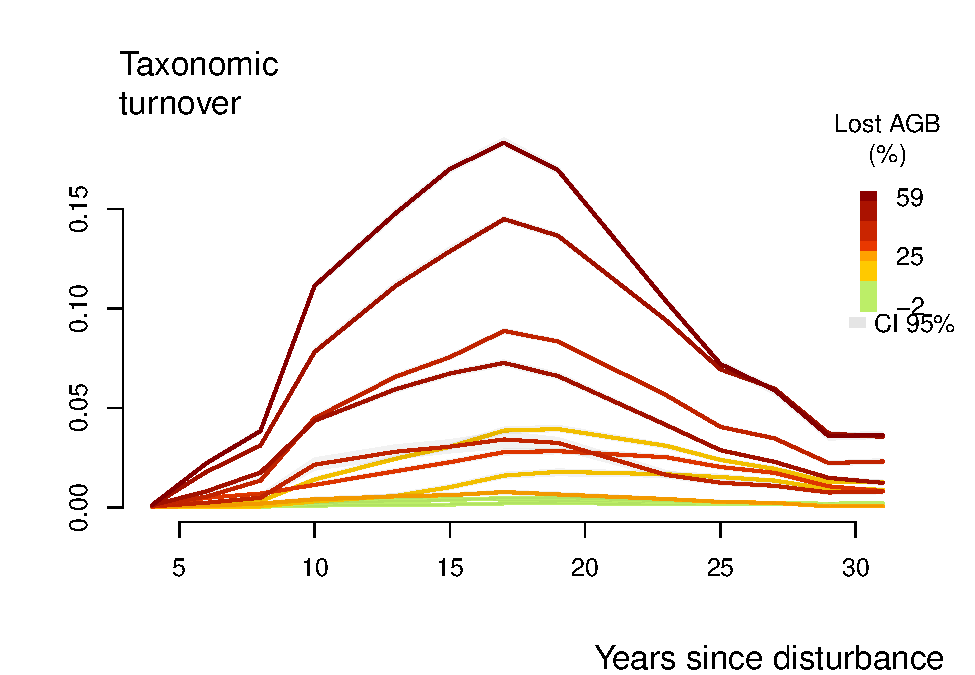
\includegraphics{RecruitmentTrajectories_files/figure-latex/Options-1.pdf}

\hypertarget{introduction}{%
\section{Introduction}\label{introduction}}

Determining the response of tropical forests to disturbance is a key to predicting their fate in the context of global climate change. In recent decades, tropical forests have experienced a wide range of disturbances, from radical land-use changes for agriculture or mining \citep{Dezecache2017a, Dezecache2017b} to more insidious changes following climate change or human activities like selective logging \citep{Baraloto2012a, Aubry-Kientz2015}.
In that respect a vast literature has successfully modeled community response to disturbance in terms of tree growth, tree height and fluxes of carbon, water and nutrients \citep{Gourlet-Fleury2000, Putz2012, Piponiot2016, Rutishauser2016}.
Tree community diversity and composition, however, proved more complex to predict as both deterministic and stochastic processes drive forests succession \citep{Norden2015}.
Deterministic successional pathways, hypothesized to follow the variations in resource availability, would involve a succession of recruitment processes depending on the species use of resources and competitive abilities \citep{Clements1916, Meiners2015}.
Such deterministic succession would shape predictable trajectories gradually restoring the pre-disturbance state of the community \citep{Chesson2000, Rees2001, Adler2007}.
Specifically, for tree species communities, deterministic pathways would first involve the recruitment of saplings benefiting from higher resources availability and reduced competition. Then, stand maturation would progressively enforce the exclusion of low-competitive species until early-successional species are replaced by late-successional ones driving towards the recovery of pre-disturbance composition and diversity \citep{Denslow2000}.
Along with deterministic recruitment, stochastic processes are known to drive tree community response to disturbance.
Stochastic processes would imply a much higher variability of post-disturbance trajectories \citep{Brokaw2000, Norden2015}, and may lead towards new equilibrium states instead of fully recovering their pre-disturbance state \citep{Hubbell2001, Chave2004}.
The relative importance of stochastic and deterministic processes largely depends on the environmental and historical context \citep{Chazdon2008, Norden2015}.
In the very diverse tropical forests, several studies revealed predictable and homogeneous successional patterns restoring pre-disturbance community characteristics \citep{Norden2009, Letcher2015}, while other revealed diverging post disturbance trajectories and different equilibrium states \citep{Longworth2014}.
Various entangled processes determine tree community dynamics. Among them, recruitment is crucial for the maintenance of community diversity and composition, and may also be an important source of variability \citep{Grubb1977, Hurtt1995, Clark1998}.
We aimed here to assess the relative importance of stochastic and deterministic recruitment processes in the response of a Neotropical forest to disturbance, and its recovery towards pre-disturbance state.

Two major facets of communities description are their taxonomic characteristics, corresponding species composition and diversity, and their functional characteristics, accounting for species ecology and functioning \citep{Macarthur1967, Violle2007b, Kunstler2016}.
Deterministic processes correspond to a recruitment depending on species competitive ability determined by their functional characteristics \citep{Rees2001, Perronne2017}.
Light being hypothesized as the limiting resource in tropical forests, deterministic processes are thought to drive functional succession from fast-growing species with ``acquisitive'' resource use, capable of significant and rapid acquisition of light, to slow-growing, long-lived species with ``conservative'' resource use \citep{Denslow1980, Molino2001, Bongers2009}.
Deterministic processes might be revealed by community functional trajectories regarding key leaf, wood and life-history functional traits assessing species ecology resources acquisition strategy \citep{Wright2004, Chave2009b, Herault2011}.
Stochastic processes, in turn, which correspond to a species recruitment independent of their functional characteristics would translate into random taxonomic trajectories unrelated functional trajectories.
A combination of taxonomic and functional approaches could thus reveal both deterministic and stochastic recruitment processes driving community response to disturbance \citep{Fukami2005, Chalmandrier2015, Cequinel2018}.

Here, we followed recruitment trajectories in a 75-ha cumulated area of Neotropical forest plots subject to a gradient of disturbance intensity, between 10\% and 60\% of above-ground standing biomass removed. We examined community composition, richness, evenness, and turnover of recruited trees over 30-year and compared to the pre-disturbance community. We considered both taxonomic aspects, accounting for tree species diversity and composition, and functional aspects, accounting for seven major leaf, stem, and life-history traits. We compared the recruitment trajectories with neutral models corresponding to stochastic recruitment and a randomization of species functional traits. Specifically, we (i) elucidated the role of deterministic and stochastic processes along post-disturbance successional pathway, and (ii) clarified the return of recruitment processes to pre-disturbance values of taxonomic and functional diversity and composition.

\hypertarget{material-and-methods}{%
\section{Material and Methods}\label{material-and-methods}}

\hypertarget{study-site}{%
\subsection{Study Site}\label{study-site}}

The Paracou station is located in a lowland tropical rainforest in French Guiana (5\textdegree 18' N and 52\textdegree 53' W). The climate is tropical wet with mean annual precipitation averaging 2,980 mm.yr-1 (30-yr period) and a 3-month dry season (\textless{} 100 mm.mo\_\{-1\}) from mid-August to mid-November and a one-month dry season in March \citep{Wagner2011}.
The mean annual temperature is 26\textdegree C. Elevation ranges from 5 to 50 m. Across all the study plots, the topography mainly corresponds to hilltops or hillsides, while bottomlands account for less than 1\% of the area. The plots contain shallow ferralitic acrisols over a layer of transformed saprolite with low permeability and lateral drainage. Soil conditions are homogeneous, with the exception of the highest hilltops where the thick surface soil layer allows free vertical drainage \citep{Gourlet-Fleury2004}.
The experiment comprises a network of twelve 6.25 ha plots (Table 1) that underwent three disturbance treatments in 1987 in a randomized plot design \citep{Herault2018}.
The experiment comprised three replicates of three silvicultural treatments (hereafter referred to as plots T1, T2 and T3) and three control plots (T0). All the treatments (T1, T2 and T3) included the logging of 10 trees/ha with 50 cm minimum DBH that belonged to a set of 58 commercially exploited species \citep{Gourlet-Fleury2004}.
Treatment T2 additionally comprised thinning by poison-girdling of non-commercially exploited, randomly selected species with an average 30 trees/ha with 40 cm minimum DBH. Trees subjected to poison-girdling were left standing in the plots. Treatment T3 also included logging of 15 trees/ha with 40 cm minimum DBH and the poison-girdling of 20 trees/ha with a 50 cm minimum DBH, all non-commercial species. Considering the silvicultural treatments and the resulting damage, disturbance intensity was measured as the percentage of aboveground standing biomass of trees above 10 cm DBH (\%AGB) lost between the first inventory in 1984 and that conducted five years after the disturbance \citep{Piponiot2016} estimated using the BIOMASS R package \citep{Rejou2017, Biomass2018}, and without accounting for lianas. The three treatments formed a disturbance intensity gradient with increasing loss of above-ground biomass (AGB) and increasing surface area disturbed.

\begin{table*}[t]

\caption{\label{tab:Tab1}Intervention table, summary of the disturbance intensity in the 4 plot treatments in Paracou. DBH stands for diameter at breast height and AGB for aboveground standing biomass of trees above 10 cm DBH.}
\centering
\begin{tabu} to \linewidth {>{\raggedright}X>{\raggedright}X>{\raggedright}X>{\raggedright}X>{\raggedright}X}
\toprule
Treatment & Timber & Thinning & Fuelwood & \%AGB lost\\
\midrule
Control & - & - & - & 0\\
T1 & DBH $\geq$ 50 cm, commercial species, $\approx$ 10   $trees.ha^{-1}$ & - & - & $[12-33]$\\
T2 & DBH $\geq$ 50 cm, commercial species, $\approx$ 10  $trees.ha^{-1}$ & DBH $\geq$ 40 cm, non-valuable species, $\approx$ 30   $trees.ha^{-1}$ & - & $[33-56]$\\
T3 & DBH $\geq$ 50 cm, commercial species, $\approx$ 10  $trees.ha^{-1}$ & DBH $\geq$ 50 cm, non-valuable species, $\approx$ 15  $trees.ha^{-1}$ & 40 cm $\leq$ DBH $\leq$ 50 cm, non-valuable species,\ $\approx$ 15 $trees.ha^{-1}$ & $[35-56]$\\
\bottomrule
\end{tabu}
\end{table*}\ignorespacesafterend

\hypertarget{inventories-protocol-and-dataset-collection}{%
\subsection{Inventories Protocol and Dataset Collection}\label{inventories-protocol-and-dataset-collection}}

Dominant families in the study site are Fabaceae, Chrysobalanaceae, Lecythidaceae and Sapotaceae. All trees above 10 cm DBH were mapped and measured annually since 1984. The trees are first identified with a vernacular name attributed by the forest worker team, and subsequently with a scientific name assigned by botanists during regular botanical campaigns.
Botanical campaigns have been carried out at five to six-year intervals starting in 2003, but identification levels varied between campaigns. The variability of protocols over time raised methodological issues as the vernacular names usually corresponded to different botanical species. This variability resulted in significant taxonomic uncertainties that had to be extended to composition and diversity metrics. Uncertainty propagation was performed using a Bayesian framework that reconstructed complete inventories at species level from real incomplete ones by linking vernacular and botanical names. Vernacular names were replaced through multinomial trials based on the association probability \(\big[\alpha_1, \alpha_2,..., \alpha_N\big]\) observed across all inventories between each vernacular name \emph{v} and the species \(\big[s_1, s_2,..., s_N\big]\):

\begin{align}
M_v\Big(\big[s_1, s_2,..., s_N\big],\big[\alpha_1, \alpha_2,..., \alpha_N\big]\Big) \nonumber
\end{align}

See appendix 1 and \citet{Aubry-Kientz2013} for the detailed methodology.

We considered six functional traits representing leaf economics, leaf thickness, toughness, total chlorophyll content and specific leaf area, and stem economics, wood specific gravity and bark thickness. These traits were obtained from the BRIDGE project \footnote{http://www.ecofog.gf/Bridge/}, which allow computing functional diversity as detailed below \citep{Paine2015}.
Trait values were assessed from a selection of individuals located in nine permanent plots in French Guiana, including two in Paracou, and comprised 294 species belonging to 157 genera. Specifically, three recently-expanded leaves were collected on each tree to measure the leaf thickness, measured with a digital micrometer on three punches per leaf, the leaf toughness, measured with a digital penetrometer on three punches per leaf, the leaf chlorophyll content, measured with a SPAD meter on three points per leaf and converted with calibrations for French Guianan tropical trees \citep{Coste2010}, and the leaf specific area, computed as the ratio between leaf area measured from digital scan and dry mass measured following drying to constant mass at 50\textdegree C. Mean foliar trait values of sampled leaves were used as tree-level trait value. Trunk samples were collected at 1 m high to measure bark thickness and wood specific gravity, after removal of the bark, computed as the ratio between wood dry mass measured following 72h drying at 103\textdegree C and fresh volume measured by displacement of liquid volume. For the trait value at species level, we used the median value of several sampled trees in the database.

Whenever trait values for a species were missing in the trait dataset (the case of 10\% of the species), the missing values were filled in using multivariate imputation by chained equation \citep{Mice2011}.
To account for the phylogenetic signal in the filling process, imputations were based on samples from the same genus or from the same family. Whenever a species was not present in the dataset, it was attributed a set of trait values randomly sampled among species at the next higher taxonomic level (same genus or family).
Besides, maximum specific height was retrieved from the Mariwenn database \footnote{https://www.ecofog.gf/mariwenn/}.
The database compiles information from a vast literature on the flora of French Guiana \citep{Ollivier2007} and comprises 362 species belonging to 188 genera. As seed mass information was classified in classes, no data filling process was applied and analyses were restricted to the botanical species recorded.

All composition and diversity metrics, as detailed below, were obtained after 50 iterations of the uncertainty propagation framework.

\hypertarget{recruitment-trajectories}{%
\subsection{Recruitment trajectories}\label{recruitment-trajectories}}

Species in the community were split into surviving trees from pre-disturbance communities and trees recruited subsequently. Our observation of recruitment diversity trajectories (hereafter \(H^q_{obs}\)) and turnover started from the fifth year after disturbance, meaning we considered that tree mortality induced by disturbance had ended \citep{Piponiot2016}. Trajectories then considered the trees recruited at 2-years intervals (i.e.~for date Y, the trees that were under 10 cm DBH at Y-1 but above 10 cm DBH at Y). For control plots, recruitment trajectories based on the new recruits from the year when disturbance was applied in other plots.

Trajectories of taxonomic diversity, corrected by the uncertainty propagation process, were assessed through species richness and evenness (the Hill number translation of the Simpson index) \citep{Chao2015, Marcon2015}.
The two diversities belong to the set of Tsallis or generalized entropy, respectively corresponding to the zero and two order q of diversity that emphasizes species with the species stem density. These two metrics assess community richness and evenness, which in turn, reveal the structure of dominance in the community and allowed us to assess changes in community abundance distribution.
The two diversity metrics will directly be refered as richness and evenness thereafter.
The two diversity metrics are complementary for the detection of changes in community structure \citep{Magurran2004}, and will directly be referred to as richness and evenness thereafter.

Functional diversity trajectories were assessed using the Rao index of quadratic entropy, which combines species abundance distribution and average pairwise dissimilarity based on all functional traits:

\[H_\Delta(P) = \sum_{s'}\sum_{s''}p_{s'}p_{s''}d_{s's''}\]
With \(p_{s'}\) \(p_{s''}\) the frequency of species \(s'\) and \(s''\) in the community \(P\), and \(\Delta\) the functional dissimilarity matrix which elements \(d_{s's''}\) are the euclidean distance between species measured from species trait values.

Functional composition trajectories were assessed through community weighted means (CWM) of functional traits. CWM are average trait values in the community weighted by the species relative abundance of the number of stems \citep{Diaz2007} (Figure 2).
A table of trait correlations is provided in supplementary material (Table S1) for a better overview of the trade-offs among traits.
The taxonomic similarity between recruited trees and the pre-disturbance community was measured with the relativized abundance replacement measuring species turnover between communities \citep{Podani2013a}:

\begin{equation}
T_{ab}=\frac{\sum_{i=1}^{n}|x_i^a - x_i^b| - \bigg| \sum_{i=1}^{n}{x_i^a} - \sum_{i=1}^{n}{x_i^b} \bigg|}{\sum_{i=1}^{n}\max{\left( x_i^a;x_i^b \right)}}
\label{eq:formNestedness}
\end{equation}

With \(T_{ab}\) the turnover between communities \(a\) and \(b\), \(n\) the total number of species in the two communities and \(x_{i}^{j}\) the abundance of species \(i\) in community \(j\).

Spearman correlation tests assessed the correlations between percentage of AGB lost following disturbance and diversity and composition changes. Specifically, changes in taxonomic richness, taxonomic evenness, and functional richness were assessed as the maximum difference over the 30 years between observed and pre-disturbance values and between observed and null models values. Changes in taxonomic turnover were assessed as the maximum taxonomic turnover value over the 30 years.

The observed recruitment trajectories were compared to null trajectories obtained from the taxonomic and functional null models detailed below. A taxonomic null model was built independently for each plot and each year. Taxonomic null trajectories were simulated by randomizing the (trees x plots) matrix. Recruited trees were randomly sampled in the current living community, according to the observed number of recruits. This model aimed to simulate a random assemblage of species, \emph{i.e.} regardless of species trait values, without questioning the manifold processes that shape community diversity distribution. Functional null trajectories were simulated by randomizing the (species x trait) matrix. Combinations of trait values were randomly re-assigned among species. The functional null models maintained the community abundance distribution while randomizing the relative abundance of trait values \citep{Mason2013}.
Trajectories of null diversity (hereafter \(H^q_{null}\)) were similarly obtained after 50 iterations of the random sampling models.
For each iteration of the null model, we computed the difference between null and observed trajectories. The 50 iterations made it possible to calculate a 95\% confidence interval of the difference between null and observed trajectories.

Post-disturbance diversity, composition, and turnover trajectories were analyzed via breakpoints analysis to detect the shifts in community post-disturbance response. We fit linear regression models to the trajectories, segmented according to one or two varying shifting times. The segmented models with the lower mean square error were retained for each trajectory.

\hypertarget{results}{%
\section{Results}\label{results}}

\hypertarget{taxonomic-richness-and-evenness-and-functional-diversity}{%
\subsection{Taxonomic richness and evenness, and functional diversity}\label{taxonomic-richness-and-evenness-and-functional-diversity}}

The average number of recruited trees per plot and per year throughout the survey increased with increasing disturbance intensity. Over the 30-year period, across the 12 plots, recruited trees belonged to 602 different species. Among these species, 26\% only occurred in one plot and 7\% occurred in all plots.

The analysis framework handling botanical uncertainties returned the estimation and significance of the diversity metrics: overall, the 95\% confidence interval remained below 10\% of the estimated value. As visualized in the figures, taxonomic diversity estimations showed significantly distinct trajectories among plots with no overlapping confidence intervals (Figure \ref{fig:DivTraj} a \& b). Functional trajectories were not as distinctly separated, but the confidence intervals also comprised the variability associated with the estimation of missing functional trait values (Figure \ref{fig:DivTraj} c).

In undisturbed communities, the taxonomic richness and evenness of the recruited trees remained stable over the 30-year period, with values equivalent to those of the taxonomic null model (Figure \ref{fig:DivTraj}).

In disturbed communities, the taxonomic richness followed hump-shaped trajectories first increasing and reaching maximum after around 15 years. This maximum was positively correlated with disturbance intensity (\(\rho^{Richness}_{spearman}=0.87\)).
Taxonomic richness then decreased and recovered pre-disturbance values after 30 years.
Compared to the null models, the observed taxonomic richness in disturbed plots was significantly lower than the richness of random species recruitment. The confidence interval of the difference between observed and null models remained well under zero in all disturbed plots.
In all disturbed communities, the taxonomic evenness decreased whenever the disturbance intensity over the 30 years, but the maximum decrease was weakly correlated with disturbance intensity (\(\rho^{simpson}_{spearman}=0.03\)).
Compared to the null model, the observed taxonomic evenness was significantly lower than the evenness of a random species recruitment. The difference between the observed and null model evenness followed a hump-shaped trajectory where maximum difference was reached around 25 years after the original disturbance. The maximum difference with null model was positively correlated with disturbance intensity regarding taxonomic richness (\(\rho^{Richness}_{spearman}=0.83\)), and evenness (\(\rho^{Simpson}_{spearman}=0.45\)).
The confidence interval of the difference between null and observed trajectories remained well below zero in all the disturbed plots.
The shifting point analysis of taxonomic richness and evenness trajectories revealed a single shifting point for both trajectories, occurring for disturbed communities between 15 and 20 years following disturbance for the taxonomic richness and between 10 and 23 years following disturbance for taxonomic evenness (Supp Mat, Fig.S1).

The functional diversity in the undisturbed plots remained stable and equivalent to that of the functional null model over the 30-year period. In the plots with the least disturbance, functional diversity remained stable or increased slightly and was higher than that of the null model in two of the T1 plots.
The maximum change in community functional diversity over the 30 years was positively correlated with the disturbance intensity (\(\rho^{FunctionalDiversity}_{spearman}=0.64\)).
In disturbed plots with higher disturbance intensity (T2 and T3), functional diversity decreased until 15 years after disturbance, and then started to recover initial values. The observed functional diversity remained lower than that of the null model over the 30-year period.
However, the difference between null and observed functional trajectories was only significant in the most highly disturbed plots (T3). The maximum difference between observed and null trajectories was positively correlated with the disturbance intensity (\(\rho^{FunctionalDiversity}_{spearman}=0.68\)).
The shifting points analysis of functional diversity revealed a single shifting point occurring from 10 to 23 years following disturbance (Supp Mat, Fig.S1).

\begin{figure*}

{\centering 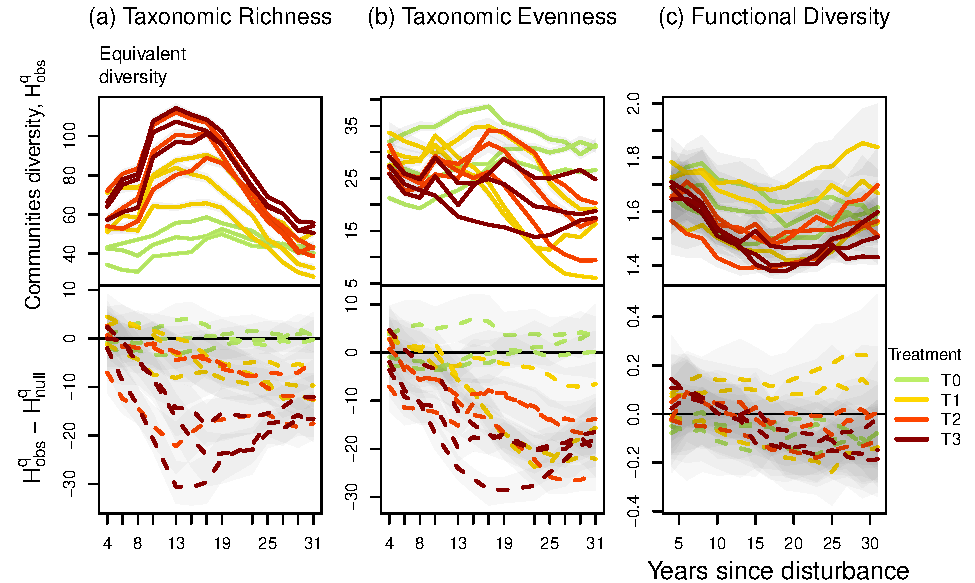
\includegraphics{RecruitmentTrajectories_files/figure-latex/DivTraj-1} 

}

\caption{Trajectories over 30 years of taxonomic richness \textbf{(a)}, taxonomic evenness \textbf{(b)}, and functional diversity \textbf{(c)} of the populations recruited at 2-year intervals. Colored lines stand for the disturbance treatment. Upper panels show observed at plot level, $H_{obs}^q$, and the lower panels show the difference between observed values and null values models $H_{obs}^q - H_{null}^q$. Shaded areas are the 95\% confidence intervals measured from the 50 iterations of the null models, when not visible on the figure, intervals are too small to be viewed}\label{fig:DivTraj}
\end{figure*}

\hypertarget{species-composition}{%
\subsection{Species composition}\label{species-composition}}

In all, 602 species were recorded over the 30 years of inventory and across the 12 plots. Among species, 157 were only inventoried in one plot and 43 were inventoried in all plots.
The detailed species distribution and the complete list of species inventoried is provided in supplementary material are presented in supplementary material (Table S2 and Table S3). The dominant recruited species were \emph{Lecythis persistens}, \emph{Licania alba}, \emph{Oenocarpus bataua}, \emph{Oxandra asbeckii}, and \emph{Eperua grandiflora}.
The dominant species recruited in disturbed plots were \emph{Miconia tschudyoides}, \emph{Inga sp.}, \emph{Oenocarpus bataua}, \emph{Licania alba}, and \emph{Xylopia sp.}.
We besides analyzed the dominant species of recruited communities in disturbed plots, considering for each plot the years before the shifting point on the one hand, and the years after the shifting point on the other hand.
During the years before shifting, the dominant species recruited in disturbed plots were \emph{Vismia} spp., \emph{Cecropia obtusa}, \emph{Oxandra asbeckii}, \emph{Cecropia sciadophylla}, and \emph{Lecythis persistens}. From the years following the shifting point, the dominant species were \emph{Miconia tschudyoides}, \emph{Miconia acuminata}, \emph{Oenocarpus bataua}, \emph{Oxandra asbeckii}, and \emph{Xylopia nitida}.

\hypertarget{functional-composition}{%
\subsection{Functional composition}\label{functional-composition}}

Functional traits in undisturbed plots remained stable over the 30-year period whereas in all the disturbed plots, with the exception of leaf chlorophyll content, the trajectories were hump-shaped. The trajectories of SLA and bark thickness initially increased before decreasing towards initial values. Conversely, trajectories of leaf thickness, leaf toughness, wood specific gravity, and maximum height first decreased and then started returning to their initial values but their recovery was still not complete at the end of the 30-year period (Figure \ref{fig:CWM}).

\begin{figure*}

{\centering 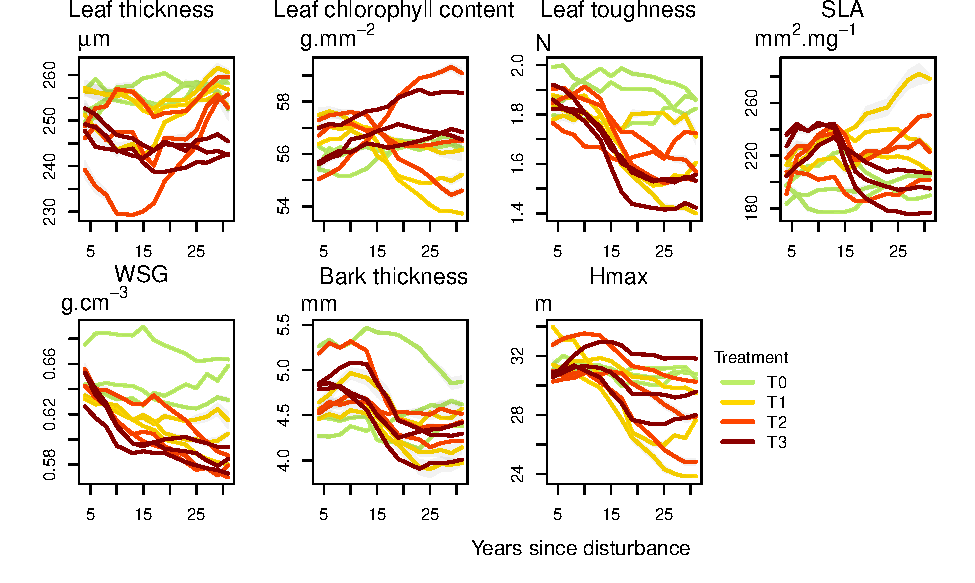
\includegraphics{RecruitmentTrajectories_files/figure-latex/CWM-1} 

}

\caption{The trajectories of community weighted means (CWM) over the 30-year period of the seven functional traits measured in the populations recruited by 2-laps. Lines represent the observed trajectories at plot level and the colors stand for the disturbance intensity. From top left to bottom right, the graphs correspond to leaf thickness, leaf chlorophyll content, leaf toughness, specific leaf area (SLA), wood specific gravity (WSG), bark thickness and maximum height at the adult stage (Hmax).}\label{fig:CWM}
\end{figure*}

\hypertarget{recruitment-turnover}{%
\subsection{Recruitment Turnover}\label{recruitment-turnover}}

The turnover of recruited species in control plots compared to the initial community remained low over the 30-year period (Figure \ref{fig:Turnover}).
In disturbed plots the turnover of the recruited species followed a marked hump-shaped trajectory, with a maximum reached about 15 years after the disturbance. The maximum turnover was positively correlated with disturbance intensity (\(\rho_{spearman}=0.93\)).
The shifting points analysis of taxonomic turnover revealed a single shifting point occurring from 17 to 23 years following disturbance (Supp Mat, Fig.S1).
Thirty years after the disturbance, the turnover had returned to low values.

\begin{figure}

{\centering 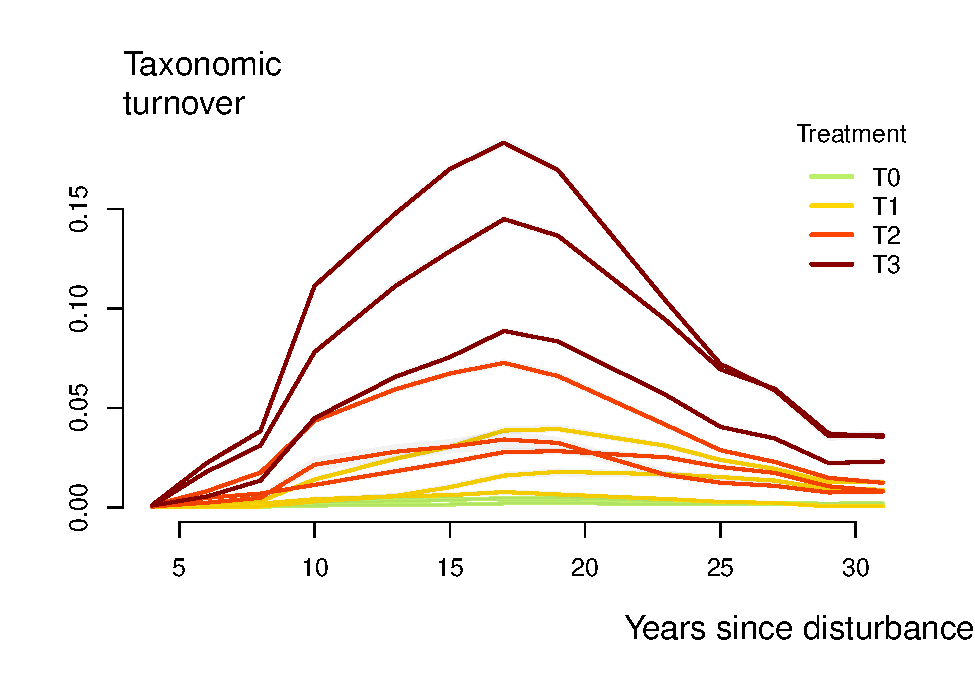
\includegraphics[width=1\linewidth]{RecruitmentTrajectories_files/figure-latex/Turnover-1} 

}

\caption{ Trajectories over the 30 years of the relativized abundance-based turnover between recruited populations and the pre-disturbance communities. Recruited populations were analyzed at 2-year intervals at plot level and compared to the plot inventory carried out before the disturbance. The colored lines stand for the disturbance treatments.}\label{fig:Turnover}
\end{figure}

\hypertarget{discussion}{%
\section{Discussion}\label{discussion}}

\hypertarget{the-emergence-of-deterministic-successional-pathway}{%
\subsection{The emergence of deterministic successional pathway}\label{the-emergence-of-deterministic-successional-pathway}}

The post-disturbance trajectories were analyzed through the botanical uncertainty propagation framework that proved accurate enough to significantly discriminate the different taxonomic trajectories, and to analyze the trends in functional trajectories.

Our taxonomic and functional analysis of recruited communities showed that following disturance, recruited communities were dominated by pioneers and light-demanding species while shade-tolerant, late successional species were dominant in undisturbed communities.
Post-disturbance recruitment trajectories followed a two-phased successional pathway defined by the emergence of deterministic competition for light temporarily offsetting the stochastic processes predominant in undisturbed communities \citep{Clements1916, Denslow2000, Meiners2015}.

A first phase was defined by the gradual increase of the taxonomic turnover between recruited trees and initial communities (Figure \ref{fig:Turnover}) and the divergence between observed and null model trajectories (Figure (\ref{fig:DivTraj}).
The first phase would correspond to a less stochastic recruitment, \emph{i.e.} deterministic, which taxonomic composition diverged from the pre-disturbance, undisturbed community.
In the first place, recruited species comprised both pioneers, like \emph{Cecropia obtusa}, and late-successional species, like \emph{Lecythis persistens} or \emph{Licania alba} corresponding to the growth of pre-disturbance surviving saplings (with DBH \textless{} 10 cm).
These saplings were the first to benefit from the reduced competition and the increased light availability following disturbances and fostering plant productivity and growth \citep{Monteith1972, Chazdon1984}.
Then, recruited species became mainly pioneers, belonging to \emph{Cecropia} or \emph{Vismia} genera, or non-pioneer light demanding species belonging to \emph{Miconia}, \emph{Oxandra}, or \emph{Xylopia} genera.
Until 15-20 years following disturbance, recruitment processes were modified by the emergence of deterministic processes favoring a restricted pool of pioneers and light-demanding species resulting in a decrease of the taxonomic richness and evenness of recruited communities.
The relative importance of these deterministic processes offsetting the stochastic recruitment of undisturbed communities increased with the disturbance intensity \citep{Bongers2009}.
Along with the decrease in recruited communities taxonomic richness and evenness, the functional composition shifted from a random trait assembly to more ``resource-acquisitive'' functional strategies (Figure 2).
Recruits specifically displayed higher light acquisition efficiency, \emph{i.e.} high SLA and low maximum height, leaf toughness and wood specific gravity \citep{Wright2004, Chave2009b, Herault2011}.
This shift towards ``light acquisitive'' functional strategies was coherent with the assumed role of light availability in the post-disturbance successional pathways, as already demonstrated in temperate and tropical forests \citep{Pena2008, Carreno2012, Kunstler2016, Both2019}.

\hypertarget{return-towards-pre-disturbance-recruitment-processes}{%
\subsection{Return towards pre-disturbance recruitment processes}\label{return-towards-pre-disturbance-recruitment-processes}}

Following the first recruitment phase, until 15 to 20 years depending on the disturbance intensity, recruitment trajectories showed a return towards pre-disturbance values of functional diversity and taxonomic richness, while taxonomic evenness and functional composition remained altered (Figure (\ref{fig:DivTraj}) \& (\ref{fig:CWM})).
Although pioneers and light-demanding species, like those belonging to \emph{Inga} or \emph{Miconia} genera, remained dominant in recruited communities late-successionals, like \emph{Licania alba}, progressively established \citep{Fortunel2014}.
The recruitment of late-successionals could reflect the progressive closing of the forest canopy and the increase in competition for light and space \citep{Peet1992, Denslow2000}. Deterministic recruitment processes, in turn, would be offset by stochastic recruitment characteristic of undisturbed forest \citep{Lawton1988, Chave2004}.
A second recruitment phase then corresponded to a return toward pre-disturbance community taxonomic and functional composition and diversity states \citep{Fukami2005, Fortunel2014}.
Such return towards pre-disturbance state would mean the maintenance of community diversity and composition after disturbance. It suggested that few species absent before disturbance were recruited, in accordance with the importance of dispersal limitations among tropical tree species \citep{Svenning2005}.
The return towards pre-disturbance state would confirm previous results obtained in the Paracou experiment, conducted 10 years \citep{Molino2001} and 20 years \citep{Baraloto2012a} after disturbance.
Both studies showed the same changes in community taxonomic and functional composition but the second study, conducted later, showed lower contrasts among disturbed plots. This was interpreted as the signs of a return towards pre-disturbance states, as species detected in the first study were short-lived pioneers that did not persist until the second study.

Although community trajectories returned towards pre-disturbance states, both taxonomic and functional characteristics remained, 30 years after the disturbance, different from pre-disturbance communities and control plot values.
The higher the disturbance intensity, the more persistent the dominance of light-demanding species. Such a long-term impact raises questions for the management of tropical forests as most valuable species are late-successional species, and their exploitation would consequently require cutting cycles longer than 30 years \citep{Putz2012}.
Furthermore, persistent changes in community composition likely alter community functioning \citep{Diaz2005}, and increase the risk of losing keystone species, with unexpected ecological consequences \citep{Jones1994, Chazdon2003a}.
Infrequent species might indeed have unique functional characteristics in the ecosystem, apart from the ones considered here, or be a key resource for some of the fauna \citep{Schleuning2016}.

\color{black}

\hypertarget{conclusion}{%
\section{Conclusion}\label{conclusion}}

Post-disturbance recruitment trajectories revealed a two-phase deterministic successional pathway driven by the emergence of trait-based deterministic processes temporarily offsetting stochastic recruitment processes and favoring light-acquisitive species.
The first phase corresponded to the recruitment of a restricted pool of pioneers and light-demanding species that were favored by the emergence of competitive exclusion for light.
Above a disturbance intensity threshold, disturbed communities saw the dominance of short-lived, fast growing pioneers that drastically changed community composition, diversity, and likely functioning.
The second phase corresponded to the recovery of stochastic recruitment processes and to a shift towards pre-disturbance taxonomic and functional characteristics. Although the diversity and composition of the recruits returned towards pre-disturbance values, this took longer that 30 years after the original disturbance. Concerning forest management, our results support cutting cycles longer than 30 years and demonstrate long-term impacts, underlining the need to evaluate forest management sustainability.

\hypertarget{acknowledgement}{%
\section{Acknowledgement}\label{acknowledgement}}

We are extremely grateful to all Paracou station technicians and colleagues who helped set up the plots and collected data over the years. Without their precious work, this study would have not been possible. Our work benefited from an \emph{``Investissement d'Avenir''} '' grant managed by the Agence Nationale de la Recherche (LABEX CEBA, ref ANR-10-LBX-25).

\hypertarget{data-availability}{%
\section{Data availability}\label{data-availability}}

This article is based upon the Paracou station dataset, which is part of the Guyafor permanent plots network in French Guiana (Cirad-CNRS-ONF). The dataset is available from the scientific director (https://paracou.cirad.fr) upon request.

\begin{center}\rule{0.5\linewidth}{\linethickness}\end{center}

%----------------------------------------------------------------------------------------
%	REFERENCE LIST
%----------------------------------------------------------------------------------------

\bibliographystyle{mee}
\makeatletter
% The filename has .bib extension the must be eliminated
\filename@parse{references.bib}
% parse stores the file name in base. Extension starts at the first dot, so don't use dots in file names.
\bibliography{\filename@base}
\makeatother


%----------------------------------------------------------------------------------------

\end{document}
